\chapter{Script development \label{scriptdevelopment}}

\section{Introduction}

\important{
This chapter is not intended to be a complete tutorial on how to develop scripts in \softwarename, the only purpose is to provide a getting started. The best way of getting familiar with the script development is to study the pre--defined scripts that come with the software. Nevertheless, anyone who intends to start developing for \softwarename, should have a good knowledge of programming in another (script) language.
}

To start the development environment, you first need to make sure that no script is currently running in the software. This can be achieved by pressing Ctrl+Z repeatedly until the last script stops (note that the startup screen with the menu overview of all animations is a script by itself). You can then bring the \sourcewin\ to the top of the window stack using the Windows Alt+TAB keyboard combination.

\section{The source code window}
\begin{figure}
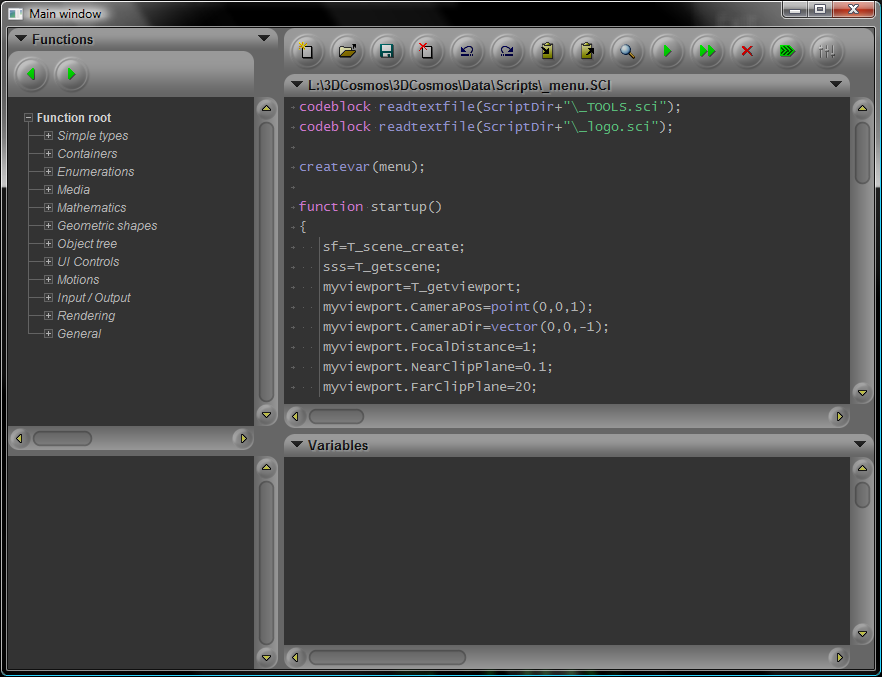
\includegraphics[scale=0.4]{bitmaps/sourcecodewindow.png}
\caption{The source code window.}
\label{sourcecodewindow}
\end{figure}
When the \sourcewin\ is opened (see \figref{sourcecodewindow}), it is divided in three different parts:
\begin{itemize}
\item On the left side, over the full height, the \functionspanel\ is shown. Underneath this panel, the \objectspanel\ is hidden. You can switch between both panel by clicking on the header, and chosing the appropriate panel name from the context menu.
\item On the top right side is the \sourcecodepanel.
\item On the bottom right side is the \varspanel. Underneath this panel, the \outputpanel\ is hidden. You can switch between both panel by clicking on the header, and chosing the appropriate panel name from the context menu.
\end{itemize}

\subsection{The \sourcecodepanel}
This panel displays the source code of the active script. The file name of the script is displayed in the header of the panel. If several scripts are loaded simultaneously, you can switch between them by clicking on the header (where the file name is displayed), and selecting another script from the context menu. The two arrows pointing down at the edges of the header indicate that more options are available at this panel, hidden behind the current view. Table \ref{sourcecodewindowcommand} gives an overview of all the commands that are available in the source code \sourcecodepanel. In addition, the script editor accepts most standard Windows keyboard shortcuts, such as Ctrl+C for Copy, Ctrl+V for paste, etc...

\begin{table}
\begin{tabular}{l p{12cm} }
\hline
Button & Description \\ \hline
BT1 & Create a new script \\
BT2 & Open an existing script \\
BT3 & Save the active script \\
BT4 & Close the active script (removing it from the \sourcecodepanel, but keeping the version on disk) \\
BT5 & Undo the last edit action \\
BT6 & Redo the last action that was undone \\
BT7 & Copy the current selection to the clipboard \\
BT8 & Paste the content of the clipboard \\
BT9 & Search for text in the active script \\
BT10 & Start the debugging of the active scipt \\
BT11 & Run the acrtiv script in debug mode \\
BT12 & Stop the execution of the script \\
BT13 & Animate the active script \\
BT14 & Open the settings dialog box \\
\hline
\end{tabular}
\caption{Commands of the code window.}
\label{sourcecodewindowcommand}
\end{table}


\subsection{The \functionspanel}
In order to assist the exploration of the rich programming environment offered by \scriptlang, this panel offers an overview of all available classes and functions, logically arranged into a tree. You can expand and collapse branches in the tree by clicking on the boxes. For each component of the function tree, the lower part of the panel gives a brief description of its functionality. This description may have hyperlinks that lead to other parts of the function tree. You can copy a specific funcion or class name into the source code by pressing the Ctrl key while clicking on the name in the tree.

\subsection{The \varspanel}
If a script is running in debug mode, this panel displays a list of all existing variables, with their content.

\subsection{The \outputpanel}
As a part of a debugging process, a script may write information to this panel using the script function \filename{output}.

\subsection{The \objectspanel}
The current state of \softwarename, including the scene(s), subframes, geometric objects that appear in these scenes, motions, textures, etc... are all maintained in a single tree structure called the \objecttree. This is a very important concept in the software, because it provides a complete description of the current state of the animation. At any time, the \objectspanel\ gives an overview of this \objecttree. In the lower part of this panel, the properties of the selected object in the tree are displayed. This panel can be used as a debugging tool to get better insight in the current state of the software.

\section{Fundamentals of \scriptlang}

\subsection{Types and variables}
\scriptlang\ shares many properties with modern script languages, such as JavaScript. Statements are separated by semicolons (\sourcecode{;}). The language is structured and object--oriented, and uses dynamic typing. This means that data types (\sourcecode{string}, \sourcecode{scalar}, \sourcecode{time}, ...) are associated with \emph{values}, and not with \emph{variables}. In addition, variables do not have to be declared explicity, since their existence is triggered by an assignment operation. For example:

\begin{lstlisting}
x="abc";
x=42;
x=time(2010,1,1,0,0,0);
\end{lstlisting}

consecutively assigns to the variable \sourcecode{x} the string "`abc"', the value 42, and a time corresponding to January 1 2010, 0h UT.

Apart from explicity assignment of a variable to a value, there are two other ways to create a variable. One is the assignment to a data type. For example, \sourcecode{mylist=list;} creates a new variable with name ``mylist'' that holds a list object. Another method is to use the function \sourcecode{createvar}, which creates a variable that is not assigned to any data content.

\important{
In \scriptlang, there is no distinction between the conventional ``float'' and ``integer'' data types: both are \sourcecode{scalar} (\ref{T:Scalar}) object types. An integer is simply a \sourcecode{scalar} with an integral value.
}

\scriptlang contains a large number of object types, that can roughly be categorized in three classes: basic object types, container object types and animation object types. A complete description of all object types is beyond the scope of this section, but the \functionspanel\ in the \sourcewin\ offers a great starting point to start exploring all available object types.

\subsection{Basic object types}
Object types that fall in this category are not necessarily simple by nature, but distinguish themselves from animation object types because they have a general meaning that makes sense outside the scope of \softwarename. The ``Simple types'' branch (\ref{Simple types}) contains conventional object types such as \sourcecode{string} (\ref{T:String}), \sourcecode{scalar} (\ref{T:Scalar}) and \sourcecode{time} (\ref{T:Time}) are present.

In addition, \scriptlang\ also knows a large amount of specific data types that can be used to perform mathematical manipulations with 3D geometry, available under the ``Mathematics'' (\ref{Mathematics}) branch of the \functionspanel. For example, there are \sourcecode{point} (\ref{T:Point}) and \sourcecode{vector} (\ref{T:Vector}) object types, but also more sophisticated concepts are available, such as the \sourcecode{LineSegment} (\ref{T:LineSegment}) and \sourcecode{Transformation} (\ref{T:Transformation}) object types.

In addition, the ``Media'' branch (\ref{Media}) of the \functionspanel\ offers a number of object types that are associated with multimedia: \sourcecode{Bitmap} (\ref{T:Bitmap}), \sourcecode{Video} (\ref{T:Video}) and \sourcecode{Sound} (\ref{T:Sound}).

\subsection{Container object types}
There are object types that serve as a container to group several objects into a single new object.
\subsubsection{List (\ref{T:List})}
A list is linear collection of objects, accessible through an index (i.e. a \sourcecode{scalar} with an integral value). Note that these components do not have to have the same object type. Individual components in a list object are addressable with the \sourcecode{()} operator:

\begin{lstlisting}
mylist(0)="abc";
mylist(1)="def";
mylist(2)=42;
mylist(10)=point(0,0,0);
result=mylist(10);
\end{lstlisting}

\subsubsection{Map (\ref{T:Map})}
A map is a collection of objects, each one identified by a unique string. As a syntax shortcut, the dot operator can be used to address the components of a map, creating a class--like syntax:

\begin{lstlisting}
mymap=map;
mp.myname="This is my name";
mp.myval=42;
mp.mypoint=point(1,2,3);
\end{lstlisting}

\subsection{Animation object types}
Under the ``Object Tree'' branch (\ref{Object tree}) of the \functionspanel, a large number of objects types is available that are used as building blocks for scenes in animations. This includes object types like \sourcecode{Subframe} (\ref{T:Subframe}), \sourcecode{Sphere} (\ref{T:Sphere}), \sourcecode{Cylinder} (\ref{T:Cylinder}), etc... Objects that belong to one of these types will automatically become member of the current \objecttree\ of \softwarename, and appear in the \objectspanel.

\subsection{Custom functions}
You can declare a custom function in \scriptlang with the \sourcecode{function} statement:

\begin{lstlisting}
function myfunction(arg1,arg2)
{
   return(arg1+arg2);
}
\end{lstlisting}

Note that \scriptlang\ is very relax in the way a custom function is declared: the object type of the argument(s) and return value is not specified. Only at run--time will the variables \sourcecode{arg1} and sourcecode{arg2} have a specific type. If the $+$ operator is defined for these types, the function will successfully return the result. If not, a run--time error will be generated.


\subsection{Including code from other locations}
You can dynamically insert code at a specific point in the script using the \sourcecode{codeblock} directive. This directive should be followed by a string or an expression that evaluates to a string. A typical example is the inclusion of the source code from another script file:

%\lstset{numbers=left, numberstyle=\tiny, stepnumber=1, numbersep=5pt}

\begin{lstlisting}
codeblock readtextfile(ScriptDir+"\_TOOLS.sci");
\end{lstlisting}

The function \sourcecode{readtextfile} (\ref{F:readtextfile}) takes a file name and returns the content of that file as a string, which is in turn inserted as code at this point by the \sourcecode{codeblock} directive.

\section{A sample animation script}

The following \scriptlang script implements a simple but operational animation, showing a rotating bar. It can be found as \filename{sample.sci} in the pre--installed set of scripts.

\begin{lstlisting}[numbers=left]
codeblock readtextfile(ScriptDir+"\_TOOLS.sci");

rootframe=T_scene_create;
root.SC.AmbientLightColor=color(0.2,0.2,0.2);

vp=T_getviewport;
vp.CameraPos=point(0,5,10);
vp.CameraDir=vecnorm(point(0,0,0)-vp.camerapos);
vp.FocalDistance=10;
vp.NearClipPlane=0.1;
vp.FarClipPlane=20;

mybarframe=rootframe.addsubframe("BarFrame");
rotation=MotionRotate.create(mybarframe,"MyRotation");
rotation.NormDir=vector(0,1,0);
mybarframe.MotionName=rotation.name;
mybar=mybarframe.add("bar");
mybar.SizeX=2;mybar.SizeY=1;mybar.SizeZ=0.5;
mybar.position=point(-1,-0.5,-0.25);
mybar.color=color(0.3,0.9,0.5);

root.time=time(2010,1,1,0,0,0);
root.timespeedfactor=1;

while true do {
   incrtime;
   render;
}
\end{lstlisting}

This script can be used as an example for how a typical script is set up. There are always two major components:
\begin{description}
\item[The setup part.] The scene is initialised and al the components of the animation are created (lines 1--23).
\item[The animation loop.] The actual rendering and animation of the scene is performed in a loop (lines 25--28). In this case, the animation loop is as simple as it can get. In general, a lot of sophistication can be put in this loop in the form of script source code.
\end{description}

Line 1 tells compiler to include the source code that is found in the script \filename{\_TOOLS.SCI} in the standard scripts directory (this is the ``Scripts'' subdirectory of the \datadir). This script contains a number of utilities that are used in almost every script.

Line 3 calls the function \sourcecode{T\_scene\_create}, which can be found in \filename{\_TOOLS.SCI}, and performes a complete initialisation of a new scene (\ref{T:Scene}), returning the default subframe (\ref{T:Subframe}) of this scene.

Line 4 sets the ambient color of the new scene (\ref{F:Scene:AmbientLightColor}).

Line 6 calls the function \sourcecode{T\_getviewport} (also present in \filename{\_TOOLS.SCI}), which returns the viewport (\ref{T:Viewport}) that was created by \sourcecode{T\_scene\_create}. This viewport is stored in the variable \sourcecode{vp}.

Line 7 sets the position of the fictitious camera that is used to record the scene (\ref{F:Viewport:CameraPos}).

Line 8 sets the viewing direction of this camera. Using elementary vector calculation, it is set in such a way that it looks at the origin (\ref{F:Viewport:CameraDir}).

Line 9 sets the ``focal distance'' or stereo baseline (see \ref{stereobaseline}) (\ref{F:Viewport:FocalDistance}).

Line 10 and 11 set the front and back clipping distances for the rendering of the scene. Anything that is closer to the camera than \sourcecode{NearClipPlane} (\ref{F:Viewport:NearClipPlane}) or further away than \sourcecode{FarClipPlane} (\ref{F:Viewport:FarClipPlane}), will not be rendered.

Line 13 creates a new subframe (\ref{T:Subframe}), that will hold the bar object and will have a motion attached to it.

Line 14 defines a rotation--style motion (\ref{T:MotionRotate}). The ``Motions'' branch (\ref{Motions})contains a list of all possible motions. Line 15 sets the rotation axis equal to the Y--axis.

Line 16 Specifies that the subframe ``BarFrame'' should be animated according to this motion (\ref{F:Subframe:MotionName}).

Line 17 Creates a bar object in the subframe (\ref{F:Subframe:add}, \ref{T:Bar}). Lines 18--20 specify the color, dimensions and position of this bar. Because this bar was created in the subframe ``BarFrame'', it will automatically follow the motion attached to this subframe.

Line 22 and 23 specify the start time of the animation (\ref{F:ObjectRoot:Time}) and the animation time multiplication factor (\ref{F:ObjectRoot:TimeSpeedFactor}). In this case, the animation runs in real time.
Line 25--28 are the animation loop. Each cycle of the loop consists in two steps: increasing the time (\sourcecode{incrtime}, \ref{F:incrtime}) and rendering the scene to the \renderwin\ (\sourcecode{render}, \ref{F:render}).

\section{The Object Tree}
The \objecttree\ is a crucial concept in writing animations for \softwarename. During the setup phase of the animation, this tree will be populated with important elements such as a scene, the viewport, subframes, geometrical objects, motions, textures, etc... Most of the required elements (the root, a single scene with a single subframe and a single viewport) are set up automatically by the helper function \sourcecode{T\_scene\_create} in \filename{\_TOOLS.SCI}.

\subsection{The Object Root}
There is always a single \term{Object Root} (\ref{T:ObjectRoot}) present. It contains a number of important properties, most of which are set automatically by the pre--defined Setup script (\ref{settings}). In addition, it also contains a number of properties that must be set by the animation, such as the current time and the time speed factor.

\subsection{Viewports}
In most animations, the \term{Object Root} will contain exactly one \term{Viewport} (\ref{T:Viewport}). A \term{viewport} contains all the information about how the scene is registered by the virtual camera for rendering to the \renderwin: the camera position, orientation and aperture, the stereo settings, the front and back clipping planes, etc... Many properties of the \term{viewport} are set by the global Settings script (\ref{settings}), but there are several important properties that need to be set by the animation script.

\subsection{Scenes}
In most animations, the \term{Object Root} will contain exactly one \term{Scene} (\ref{T:Scene}). A \term{scene} contains a number of important properties, such as the position and color of the light source(s), the background color, etc...

\subsection{Subframes}
Positions in the 3D world of a \term{scene} are defined by three coordinates $(x,y,z)$ in a orthonormal basis. When a more complex scene is built, it is often useful to define a part of it in a different basis. For example, suppose that the scene contains a car with four wheels. It is convenient to define a wheel relative to its center (preferably in a separate function), and specify where on the global scene this will should be positioned (both origin and direction). You can do this by defining a \term{subframe} (\ref{T:Subframe}), specify the basis of the coordinate system for this subframe in terms of the coordinate system of the global scene, and define the geometric objects that describe the wheel relative to this subframe. Repositioning of this wheel to a different position and/or direction on the scene then simply becomes a matter of manipulating the basis of this \term{subframe}. This can be done by accessing the property \sourcecode{Transf} (\ref{F:Subframe:Transf}), which sets or returns a \sourcecode{Transformation} object (\ref{T:Transformation}). Each scene should have at least one subframe.

\important{\softwarename\ uses homogeneous coordinates and affine transformations to describe the 3D space of a scene. A good understanding of these concepts and geometry in general is necessary to successfully write scripts that create scenes and animations.}

A \term{subframe} can belong to the \term{scene}, but it can also belong to another \term{subframe}. In this case, the basis of the new subframe is described relative to the basis of the parent subframe. In such a way, complex scenes can be described as hierarchical structures of nested \term{subframes}.

\subsection{Geometric objects}
The visible objects that build the scene are called \term{geometric objects}, and can be found in the \term{Object tree>Geometric Objects} branch of the \functionspanel. These objects can be added to a \term{subframe} using the member function \sourcecode{add} (\ref{F:Subframe:add}). Examples of such objects include spheres (\ref{T:Sphere}), cylinders (\ref{T:Cylinder}), but also text (\ref{T:Text3D}). These objects have numerous properties to define their appearance: visibility, color, texture...

\subsection{Textures}
A very powerful concept in 3D rendering are the so--called \term{textures}. This is a bitmap image that is wrapped over a geometric object, in order to give it a more realistic appearance. For example, a convincing rendering of the Earth as a planet can be created by wrapping a bitmap with a World map over a (flattened) sphere. A texture object in \softwarename\ (\ref{T:Texture}) is always member of a \term{subframe}, and can be created with the member function \sourcecode{CreateTexture} (\ref{F:Subframe:CreateTexture}). Once created, this texture can be assigned to an individual geometric object with the property \sourcecode{Texture} (e.g. \ref{F:Sphere:Texture} for Sphere objects). 

\subsection{Motions}
Many animations show moving objects. Usually, this is achieved by placing a moving object in a \term{subframe}, and change the move the basis that define this subframe with respect to its parent. There are two different approaches to achieve this:
\begin{enumerate}
\item In the render loop, calculate and set the new position of the subframe each time before rendering a new frame.
\item In the setup phase, define a \term{motion} that controls how the subframe is moving during the animation, and attach this motion to the corresponding subframe.
\end{enumerate}
The second option has the advantage that the source code of the script is usually simpler and easier to understand, and that the rendering may be faster because the pre--defined motions are optimised for calculation speed. The first option offers maximum flexibility, but is often harder to program. The ``Motions'' branch in the \functionspanel enumerates a list of all possible motions (see also \ref{Motions}).

Note that a motion can not only control the position of a \term{subframe} (i.e. the origin of its basis), but also its complete 3D orientation (i.e. the orientation of its orthogonal basis with respect to the parent subframe). A \term{motion} can apply a general \term{affine transformation} to the subframe (\ref{T:Transformation}). For example, a \sourcecode{MotionRotate}) object (\ref{T:MotionRotate}) causes a subframe to spin around a given axis, at a specific rotation speed.